\subsection{Data Collection}
The data taken was for the variables in equation \ref{eq:NozzleForce}. There were a total of 10 nozzle expansion ratios used with 2 trials each. The expansion ratio kept $A_t$ constant and varied $A_e$. There were 4 over expanded, 4 underexpanded, 1 optimum, and 1 with no expansion. The naming scheme goes something like ERT, where E stands for either U (Underexpanded), N (None), or O. O stands for either optimum or overexpanded. R is the ratio number (1-4) except in the case that there is no third character. In this case the O stands for optimum, which there is only one of. T stands for trial number which can be either 1 or 2. So for example, U22 is underexpanded, ratio number 2, trial number 2. O1 is optimum ratio, trial number 1. These are explicitly defined in the nomenclature section.%
\nomenclature{$O11$}{Overexpanded area ratio 1, trial 1}%
\nomenclature{$O12$}{Overexpanded area ratio 1, trial 2}%
\nomenclature{$O21$}{Overexpanded area ratio 2, trial 1}%
\nomenclature{$O22$}{Overexpanded area ratio 2, trial 2}%
\nomenclature{$O31$}{Overexpanded area ratio 3, trial 1}%
\nomenclature{$O32$}{Overexpanded area ratio 3, trial 2}%
\nomenclature{$O41$}{Overexpanded area ratio 4, trial 1}%
\nomenclature{$O42$}{Overexpanded area ratio 4, trial 2}%
\nomenclature{$U11$}{Underexpanded area ratio 1, trial 1}%
\nomenclature{$U12$}{Underexpanded area ratio 1, trial 2}%
\nomenclature{$U21$}{Underexpanded area ratio 2, trial 1}%
\nomenclature{$U22$}{Underexpanded area ratio 2, trial 2}%
\nomenclature{$U31$}{Underexpanded area ratio 3, trial 1}%
\nomenclature{$U32$}{Underexpanded area ratio 3, trial 2}%
\nomenclature{$U41$}{Underexpanded area ratio 4, trial 1}%
\nomenclature{$U42$}{Underexpanded area ratio 4, trial 2}%
\nomenclature{$O1$}{Optimum area ratio, trial 1}%
\nomenclature{$O2$}{Optimum area ratio, trial 2}%
\nomenclature{$N1$}{No expansion, trial 1}%
\nomenclature{$N2$}{No expansion, trial 2}
This naming scheme will be upated in future experiments because it was slightly problematic in the analysis of the data.
\begin{tcolorbox}[breakable,title=Data Sensors, height fixed for=first and middle]
There should be some light discussion on the sensors used for data collection. There was a single pressure transducer located near the inlet of the nozzle, a thermocouple located on the nozzle, a thermocouple located inside of the adaptor that the $CO_2$ connected to the rest of the plumbing, and a load cell setup to measure the thrust produced from the CGT. For sake of simplicity I will refer to these as "sensors" preceeded by the variable they measured. So, respectively, $P_c$ sensor, $T_e$ sensor, $T_c$ sensor, and $F$ sensor. Additionally, $\gamma$ is dependent on temperature, but only changes slighty in the temperature differences noticed here. In later models, $\gamma$ will be set to be a function of temperature for greater accuracy. For now it is not necessary because the force has a small dependence on $\gamma$ compared to the temperature. So, for the sake of this project $\gamma$ is a constant. The data acquisition system was running python on a RaspberryPi 3 and since all of these sensors are analog devices 2 different analog-to-digital converters (ADCs) was used to interface with the Pi. The $P_c$, $T_e$, and $T_c$ sensors interfaced with a 10-bit ADC and the $F$ sensor interfaced with a 24-bit ADC. In future experiments, a 24-bit ADC will be used for all data acquisition because of the limited resolution with the 10-bit ADC. This is especially evident with the thermocouple data. All of the python scripts for data collection are available at my \href{https://github.com/maxmhuggins/RCS_HAB/tree/master/On_Ground_Testing/Code}{GitHub repository}.
\end{tcolorbox}
The code began the experiment after all sensors were calibrated and functioning properly. Data collection ran until the force production was below a certain threshold for a predefined number of points. This would also need to be updated because often times the force sensor would lose its zero position so defining the threshold value was not so easy. A better method would be using the change in force to determine when the experiment was over. This would work well because the force is transient until the $CO_2$ was all spent. After it was over the mass of the $CO_2$ canister was measured. All of this data was written to two seperate .txt files. One included the calibration values for the sensors and changes in mass, the other included $P_c$, $T_c$, $T_e$, and $F$. The previous was not recorded in a useful format and later work had to be done to resolve this. In the future this should be updated. The latter was simply comma delimited and worked fine for reading into python for analysis. The data files can be found at this \href{https://github.com/maxmhuggins/RCS_HAB/tree/master/On_Ground_Testing/Data_and_Analysis/Experimental_Data_Analysis/Refined_Data_Files}{GitHub repository} as well.
\subsection{Initial Analysis}
To begin the analysis, simple plots were made to look at the sensor data over time. Immediately, it was found that the temperature data is quite poor! The resolution of the ADC is evident in the discrete steps that the temperature takes. Figure \ref{fig:BadTemp} shows an example of the temperature data.
\begin{figure}[h!]
\centering
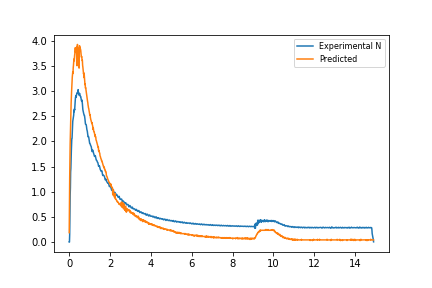
\includegraphics[scale=.5]{Figures/ExampleTemp}
\caption{Example plot of the temperature over time for a trial}
\label{fig:BadTemp}
\end{figure}
The limited resolution of the ADC can be seen quite clearly. However, this is not terribly problematic and several things can be done to smooth the curve. Since smoothing this data is not the objective here, I have simply taken a function from the pandas python library that handles smoothing quite well. It uses a moving averages method. The smoothed plot is shown in figure \ref{fig:SmoothedTemp}.
\begin{figure}[h!]
\centering
\includegraphics[scale=.5]{Figures/SmoothTemp}
\caption{Example plot now smoothed}
\label{fig:SmoothedTemp}
\end{figure}
There are additional problems that come with smoothing data, though. The total number of points is typically reduced and therefore all of the data that is going to be used must then be smoothed by the same factor. Also, the data is shifted to the left as can be seen from figures \ref{fig:BadTemp} and \ref{fig:SmoothedTemp}. Alternatively, a function could be fit to the data and this would allow the possibility of a continuous data set. For now though, there are bigger problems with the data recorded. Figure \ref{fig:BothTemps} shows the two different temperature data sets plotted against time for one of the trials. 
\begin{figure}[h!]
\centering
\includegraphics[scale=.5]{Figures/TwoSmoothedTemps}
\caption{Smoothed $T_c$ and $T_e$ plotted with time for one of the trials}
\label{fig:BothTemps}
\end{figure}
It can be seen immediately that at some point the $T_c$ line drops below the $T_e$ line. Looking back at equation \ref{eq:NozzleForce} this is troublesome. This means that $\left(1-\frac{T_e}{T_c}\right)<0$ giving an overall negative sign under the square root. Obviously the force produced is not imaginary, so either the data collected for these temperatures is not representative of the actual variables or the theory is wrong. It is obvious that the former is the problem for several reasons. The first is that the $T_c$ variable represents the temperature directly before the converging section of the nozzle. $T_e$ is the temperature of the exit plane of the nozzle. The two thermocouples are not placed in these regions. Admittadely, there was not enough attention when inspecting the theory to develop the experiment. Under normal circumstances some simple changes would be made and new data would be taken, however due to the closure of the university nothing can be done about collecting new data. Because of this we will proceed with what analysis can be completed and use a more general approach to characterizing the CGT. First, I've plotted the predicted force with the experimental force in figure \ref{fig:FirstThrust}. 
\begin{figure}[h!]
\centering
\includegraphics[scale=.5]{Figures/FirstAttempt}
\caption{First attempt at plotting the thrust and predicted thrust against time}
\label{fig:FirstThrust}
\end{figure}
As expected, we see segments where the force is undefined due to a runtime error in the numpy package. What can be done here? Well, some more consideration should be taken into the theory. Starting with a gas obeying the ideal gas law in an adiabatic system.

after some substitution we can obtain \ref{eq:PtoT}.
\begin{equation}\label{eq:PtoT}
\left(\frac{P_x}{P_{x+dx}}\right)^{\frac{\gamma-1}{\gamma}}=\frac{T_x}{T_{x+dx}}
\end{equation}
now, if $P_x=P_c$ and $P_{x+dx}=P_e$, we can look at this negative sign more intuitively. We know that a nozzle will never function properly in a state where the exit plane pressure is less than the chamber pressure. Also, since the $\gamma$ value is always greater than 1, the overall term will be greater than 1 which means the exit plane temperature must always be less than the chamber temperature. In other words, we know $P_c>P_e$ and $\gamma>1$ therefore, $\left(\frac{P_c}{P_e}\right)^{\frac{\gamma-1}{\gamma}}>1$ which also means $T_c>T_e$ always. Additionally, since gases cool as they expand, it is sensible that the chamber will be warmer than the exit plane of the nozzle.\\
At this point, confidence has been established in the theory and changes should be made to the experimental setup. Again, unfortunately, these changes cannot be made but we will continue with the analysis regardless.
\subsection{Attempt at Reconciliation}
The most obvious way to resolve the negative sign is to include an absolute value around the problematic term. This solves the runtime error, but is unfounded. We know the optimum nozzle expansion ratio should have the largest thrust production, but we have essentially removed $T_e's$ dependence on the expansion ratio in doing this. This means the thrust will be highest for the value which has the greatest expansion ratio which is geometry O4. This can be seen in figure \ref{fig:FirstThreeCurves}. I have plotted several trials there and included the predicted force according to equation \ref{eq:NozzleForce}.
\begin{figure}[h!]
\centering
\includegraphics[scale=.5]{Figures/FirstThreeCurves}
\caption{Several trials thrust curves plotted with the predicted thrust}
\label{fig:FirstThreeCurves}
\end{figure}
O4 is indeed the largest thrust curve. Also, in viewing these thrust curves it is important to recognize the predicted force is the predicted force per unit mass, but the actual curve is per some different mass value. However, the unit for the mass can be set to some convenient unit and be compared through all the data. This won't change the actual analysis and design conditions.\\
Tacking on an absolute value will not only fail to resolve the issue here but it is also unfounded. The next thought is to solve for $T_e$ in terms of the other available variables. It turns out that $T_e$ can be put in terms of $T_c,\ P_c,\ A_e,\ \rho_c,\ and\ w$.%
\nomenclature{$w$}{Mass flow rate}
Unfortunately, there are several problems with this. The first is that the change in mass, the mass flow rate, was only measured as an initial and final value. Meaning the total mass used throughout the experiment is known, but the mass flow rate throughout is not. For now, the assumption will be made that the mass flow rate is constant. Next, as can be seen from equation \ref{eq:ExitTemp} $T_e$ cannot be solved algebraically. It is not difficult to solve for it computationally though. 
\begin{equation}\label{eq:ExitTemp}
T_e = T_c\left[\frac{\gamma -1}{2\gamma P_c \rho_c} \left(\frac{w}{A_e}\right)^2\left(\frac{T_c}{T_e}\right)^{\frac{\gamma+1}{\gamma-1}}+1\right]^{-1}
\end{equation}
The simplist method is to use the relaxation method as described in \cite{newman}. The process is to iterate the equation by plugging in $T_e=1$ on the right side, finding a new value for $T_e$ on the left side, substitutting this value back into the right side, and so on. $T_e$ should converge to a value and that is the solution for $T_e$. Using this method, I've made the same plots in figure \ref{fig:SecondThreeCurves} as in figure \ref{fig:FirstThreeCurves}.
\begin{figure}[h!]
\centering
\includegraphics[scale=.5]{Figures/SecondThreeCurves}
\caption{Several trials thrust curves plotted with the predicted thrust}
\label{fig:SecondThreeCurves}
\end{figure}
The similarity between the two figures is quite apparent. At first glance, they nearly look the same, but looking at the far right plot the theoretical curve can be seen to be different from the other. The reason for this is because the assumption made about the mass flow rate being constant through time was naive. The mass flow rate, at any point $x$  can be defined by equation \ref{eq:MassFlow}.
\begin{equation}\label{eq:MassFlow}
w_x=A_x v_x \rho_x
\end{equation}%
\nomenclature{$v$}{Gas velocity}%
\nomenclature{$X_x$}{Any variable, X at some point, x}
Both the velocity and density of the gas have dependence on pressure and temperature so $w$ is \textit{not} constant with respect to time. That is not to say it is not constant at any given time throughout the entire system, however. If $T_e$ is not represented correctly it is clear that the result is that the nozzle with the largest expansion ratio is predicted to function best because of equation \ref{eq:NozzleForce}'s dependence on $A_e$. \\
In the end, there is not much reconciliation that can be done for the poor data collection. What we can look at effectively is the experimental value for the specific impulse. Unfortunately, this won't tell much because the theoretical values cannot be calculated for the same reasons as the force. Additionally, it is not ideal to look at the specific impulse over the entire experiment because the temperature and pressure are so transient. However, since the change in mass is only known for two data points it is the best that can be done. Determining these values is a simple trapezoidal sum over all time. I've tabulated all of these in table \ref{table:Isps}.
\begin{table}[!h]
\centering
\begin{tabular}{
>{\columncolor[HTML]{C0C0C0}}c 
>{\columncolor[HTML]{EFEFEF}}c 
>{\columncolor[HTML]{EFEFEF}}c }
Geometry & \cellcolor[HTML]{C0C0C0}$Trial\ 1\ I_{sp}$ & \cellcolor[HTML]{C0C0C0}$Trial\ 2\ I_{sp}$ \\
N        & 61.1                                       & 54.0                                       \\
U4       & 58.0                                       & 44.1                                       \\
U3       & 33.5                                       & 52.8                                       \\
U2       & 62.5                                       & 60.3                                       \\
U1       & 33.9                                       & 62.6                                       \\
O        & 57.5                                       & 37.3                                       \\
O1       & 58.6                                       & 59.5                                       \\
O2       & 50.5                                       & 48.3                                       \\
O3       & 29.0                                       & 60.3                                       \\
O4       & 44.6                                       & 56.0                                      
\end{tabular}
\caption{Experimental specific impulses}
\label{table:Isps}
\end{table}
There isn't much to see here, except that the values found are close to the known values from reference \cite{anis}. The $I_{sp}'s$ dependence on temperature and pressure means that these values are meaningless without the theoretical values at the same pressure and temperature. Reference \cite{anis} is using values for the maximum possible $I_{sp}$ values.